
\chapter{單一語音離散表徵與音位的關係}

  HuBERT \cite{hsu_hubert_2021, hsu_hubert_2021-2} 和 Wav2vec 2.0 \cite{baevski2020wav2vec} 等語音基石模型的成功,不僅在語音任務上達到了前所未有的表現,還促進了語音表徵離散化的發展。由此產生的「無文字(Textless)」架構 \cite{noauthor_textless_2021, lakhotia_generative_2021, lakhotia_generative_2021-1},讓人們在處理語音訊號時,有了連續表徵以外的新選擇。離散形式的表徵可以直接應用文字領域發展的技術,如機器翻譯、生成式模型等,為語音技術帶來新的突破。另一方面,基於離散「符記(Token)」的共同形式,離散語音表徵可以更好的整合文字資料,促成多模態領域的發展。跨模態離散表徵的成功,甚至驅使影像領域也開始發展離散表徵,如探討唇語的 AV-HuBERT \cite{shi2021learning} 等等,展現了離散表徵在資料處理上的優勢。

        此外,除了技術的角度切入,這樣的技術也可以探討離散語音表徵成功背後的可能因素,以及它們與語言學對人類語音理解之間的差異,甚至是進一步利用這些技術協助更細緻的探討人類的語音現象。因此,原先在連續語音表徵上的語音學分析,也開始關注離散表徵在多大程度上能描述語音現象,將其列入考量,成為除了連續語音特徵和時頻譜之外的另一個選擇。

\section{相關研究}  

\subsection{無文字與離散語音表徵}

  自 HuBERT 帶起的研究之後,出現了愈來愈多離散表徵相關的研究\cite{10097097, abdullah23_interspeech, chang_exploration_2023, liu2024dinosr, zhang2024speechtokenizer, huang2023repcodec} 。它們在提出自己的離散表徵時,也會採取 HuBERT 的衡量方式,來驗證這些離散單元與語音中的內容及人類對語音的詮釋之間,具有一定程度的相關性,並從資訊理論(Information Theory)的角度,證明這些離散單元確實具備區分不同語音資訊的能力。

\subsection{語音學分析}

  由於語音處理本身最終是針對人類語音,因此有一群研究者通過對人類語音的理解,將這些知識應用在分析模型如何對語音訊號建構表徵之上\cite{deseyssel22_interspeech, wells_phonetic_2022, 10097097, abdullah23_interspeech} 。基於這些作品對語音離散表徵的興趣和探討,本論文也先透過過往幾個常用來分析語音表徵的方式,特別是 HuBERT \cite{hsu_hubert_2021-2} 提出的標準進行初步的分析。


\section{衡量指標}

  本次研究主要探討純度(Purity)、熵(Entropy)和相互資訊(Mutual Information,MI)等指標,這些指標在 HuBERT 中被採用 \cite{hsu_hubert_2021, hsu_hubert_2021-2},用以比對機器學習過程中得到的虛擬標註與人類標註之間的相關性(Correlation),接下來將詳細解釋這些指標的定義。

        包含聲學特徵與語音基石模型,不論採用何種方式獲得語音表徵,語音訊號皆是以音框(Frame)為基本單位進行處理。具體而言,給予一段聲音訊號,語音處理系統會將這段訊號按照固定時間切割成多個片段分別處理,這些片段的長度被稱之為時間解析度(Time Resolution)。因此,對於任意一段語句(Utterance),系統會將訊號轉換成一連串的向量 $\boldsymbol{x} = [x_1, \cdots\cdots, x_T]$ 作為語音表徵,其中 $T$ 是該段語句的音框總數,與該語句的時長成比例。其中,第 $t$ 個向量 \(x_t\) 表示第 $t$ 個音框的語音訊號內容。在離散表徵的研究中,每個語音表徵向量 $x_t$ 透過向量量化(Vector Quantization)程序,對應到編碼簿中的某個碼字 $e_{z_t}$。因此,該段語句將被表示為 $\boldsymbol{z} = [z_1, \cdots\cdots, z_T]$ 的離散單元序列。

        與此對應,藉由強迫對齊器(Forced-Aligner)或人工標註,可以獲得該段語句的音素標註(Phonetic Label)。然而,通常音素標註是以每個音位的起始至終止的時間點配上此時間段的音位類別呈現。因此,為了配合語音表徵對語句的處理方式,這段音素標註會被依照時間點對應的範圍在音框上對齊,成為 $\boldsymbol{y} = [y_1, \cdots\cdots, y_T]$ 的形式以便分析與後續處理。

        為方便具體說明,吾人從語音常用的 LibriSpeech \cite{panayotov_librispeech_2015} 公開資料集中取一段音檔\footnote{取自 train-clean-100 訓練子集,編號 89-218-0056,即編號 89 語者在章節編號 218 中第 56 句。},放上波形與音框的對照在圖 \ref{fig:enter-labelwav} 呈現。 該段語句內容為 "... what means could it..." ,上方兩個橫列為單詞標註、音位標註 \footnote{ARPABet 表示法,是以純字母表示的音位表示法。介紹音位分類的章節會對此詳細描述。音位中的數字表示重音。}。接下來四個橫列中,可以看見第三與第五個橫列將語句切割成以 20 毫秒為單位的片段,此即前面所述之音框。第三列為 HuBERT 模型分群數 100 所得之離散單元序列,而第五列則是由第二列的音位標註片段按照所對應的時間段,分別對齊到音框上的音位標註。由於音位的長度通常長於一個音框,因此在離散單元和音框音位標註在呈現上習慣將標註類別相同的音框合在一起成為長短不一但更接近時間發音的時間段,分別標在第四與第六列之上。
        \begin{figure}
            \centering
            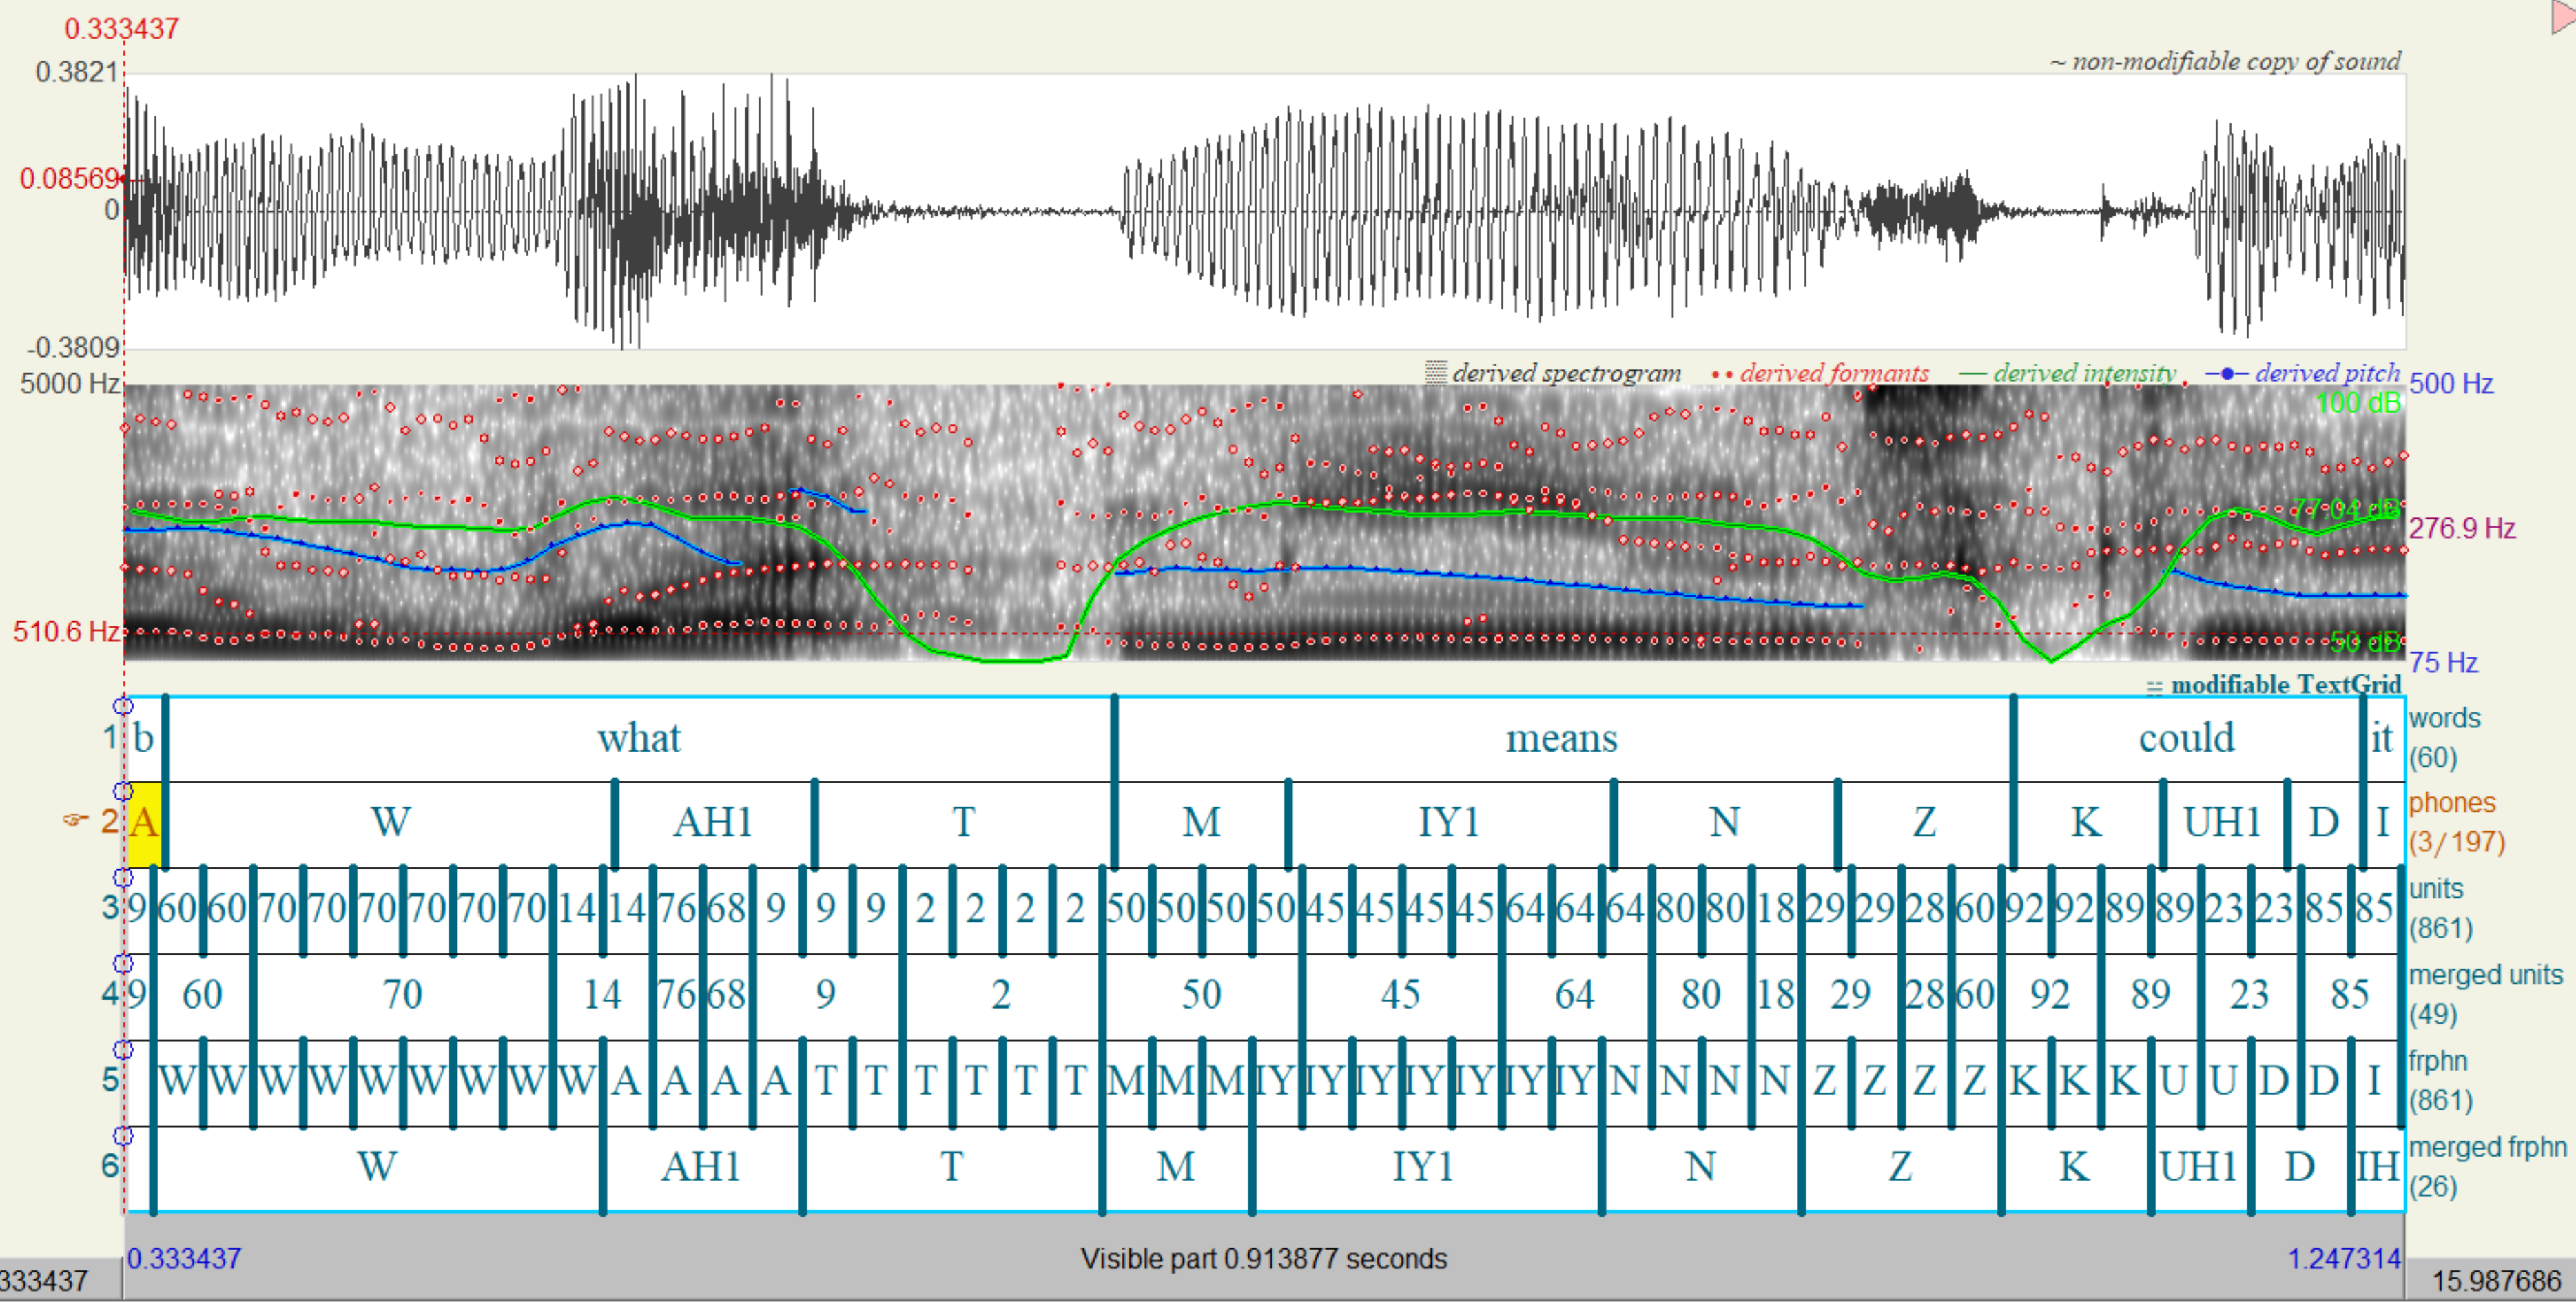
\includegraphics[width=1\linewidth]{figures/praat.png}
            \caption{以音框對齊的離散單元與音位標註範例}
            \label{fig:enter-labelwav}
        \end{figure}
        %%%%%%%%%%%%%%%%%
        
        此時若將整個待分析資料集的語音訊號全部蒐集起來,一共有 $T'$ 個音框,如此可分別獲得一個離散單元序列 $\boldsymbol{z} = \{z_t\}_{t=1}^{T'}$ 與音位標註序列 $\boldsymbol{y} = \{y_t\}_{t=1}^{T'}$ 進行統計分析。我們可以根據離散單元與標註之間配對的出現次數,寫為一個雙變數的共同分佈(Joint Distribution)
\begin{align}
    p_{yz} = \frac{\sum^{T'}_{t=1}[{y_t = i \wedge z_t = j}]}{T'}
\end{align}

其中 $i$ 是第 $i$ 個音位類別,而 $j$ 指編號為 $j$ 的離散單元。兩個變數的邊際機率(Marginal Probability)分別為
\begin{align}
    p_z(j) & =\sum_i{p_{yz}(i, j)} \\
    p_y(i) & =\sum_j{p_{yz}(i, j)}
\end{align}
因此,對於每一個音位 $i$ 而言,這個音位最可能的對應離散單元為
\begin{align}
    z^\ast(i) = \arg\max_j p_{yz}(i, j)
\end{align}
與之相對應的,對於每一個離散單元的類別 $j$ 則可以找到機率最高的音位
\begin{align}
    y^\ast(j) = \arg\max_i p_{yz}(i,j)
\end{align}
透過這些定義,以下分節介紹將要用來分析的指標。

\subsection{純度}

  本指標考慮音位和離散單元兩個序列之間對應的最高機率,因此從音位與離散單元的角度出發,可以得到以下兩項數據:

\paragraph{音位純度(Phoneme Purity)}\hfill \break
%
  考慮每個離散單元對應的音位中,最高機率音位的機率,表示為
\begin{align}
    \mathbb{E}_{p_z(j)}\left[p_{y|z}(y^*(j)|j) \right]
\end{align}
此指標表示該單元是否對其對應的音位有足夠的代表性。

\paragraph{分群純度(Cluster Purity)}\hfill \break
%
  與音位純度相對,改以每個音位的角度,考慮對應單元類別的機率
\begin{align}
    \mathbb{E}_{p_y(i)}\left[p_{z|y}(z^*(i)|i) \right]
\end{align}
        由於離散表徵進行分群演算法時的類別數是一項超參數(Hyperparameter),且通常離散單元的分群數量會比音位多,因此該統計數據本身不直接具有語音學的解釋意義,而且在分群數量很多時其數值會顯著下降。然而該指標在考量音位純度時必須一併考慮,因為當分群數非常多時,分群純度過低暗示離散單元做不到歸納音位類別的效果,使得音位純度失去其意義。一個極端的情形是每一個音框都給予不同的離散單元編號,如此音位純度可以達到 100\%。

\subsection{熵和相互資訊}

  除了純度提供「最高機率」的對應關係,根據 HuBERT 論文 \cite{hsu_hubert_2021-2} 中的分析方式,我們也可以從資訊理論的角度,觀察兩個序列的熵和相互資訊。

\paragraph{熵(Entropy)} \hfill \break
%
  熵的定義按照資訊理論,衡量兩個序列中標籤類別出現機率的不確定性(Uncertainty),公式寫作:
\begin{align}
    H(y) & = \sum_i{p_y(i)\log p_y(i)} \\
    H(z) & = \sum_j{p_z(j)\log p_z(j)}
\end{align}
其中 $H(y)$ 和 $H(z)$ 分別為音位和離散單元的熵,數值愈高分別表示各種音位和離散單元出現的機率愈平均。

\paragraph{以音位標準化之相互資訊(Phone-normalized Mutual Information,PNMI)}\hfill \break
%
  本數據以「觀察到某一個離散單元,能降低多少音位標註的不確定性」,定義該離散單元的出現背後提供了多少音位的資訊。公式寫為:
\begin{align}
    \frac{I(y;z)}{H(y)} & =\cfrac{\sum_i \sum_j p_{yz}(i, j) \log \cfrac{p_{yz}(i, j)}{p_y(i)p_z(j)}}{\sum_i p_y(i) \log p_y(i)} \\
                        & =\frac{H(y)-H(y|z)}{H(y)}                                                                              \\
                        & =1-\frac{H(y|z)}{H(y)}
\end{align}
        該項數據愈高,表示離散單元的分群愈能提供語音音位的資訊,是一個品質更好的分群結果。由於離散單元是否能夠正確對應到音位才是人們所關心的問題,因此與純度不同,只以音位的角度出發,而不考慮以離散單元分群的角度。

\section{語音學的音位分類(Phoneme Type)}

  除了單一音位本身的特性以外,由於音位之間存在相似的特徵,可以分成幾個組別。這裡依照希氏(Sicherman) \cite{10097097}、阿氏(Abdullah)\cite{abdullah23_interspeech} 等前作的分組方式,對英語的音位進行分類。如此一來,除了單純把音位標註以約 40 類完全獨立的標籤看待,還能夠觀察這些離散單元是否有擷取到相似的發聲特徵。首先,按照發音過程氣流是否受到阻礙,因此可否形成獨立的音節,音位可以分為輔音與元音兩大類,而後再根據發音的細部特性共分成七組。

\paragraph{輔音(Consonant)} \hfill \break
  
        輔音是指透過阻擋氣流發聲的音位,因此通常不單獨構成音節,
按照發音方式可分為以下五個類別:
        
        \begin{itemize}
            \item 塞音(Plosive):以完全阻塞氣流的方式發音的音位,包含 /p/、/b/、/t/、/d/、/k/、/g/ 六種。
            \item 擦音(Fricative):藉由在口腔中形成的縫隙,使氣流通過時摩擦形成的發音,包含 /f/、/v/、/s/、/z/、/\textesh/ (sh)、/\textyogh/ (如「garage」的 「-ge」)、/θ/ (無聲的 th)、/ð/ (有聲的 th)、/h/ 九種。
            \item 塞擦音(Affricate):由塞音和同部位的擦音同時發出的輔音,英語中只有 /t\textesh/ 和 /d\textyogh/ 兩種,即 ch 和 j 的發音。
            \item 鼻音(Nasal):使氣流通過鼻腔形成的聲音,有 /m/、/n/、/ŋ/ (ng) 三種。
            \item 近音(Approximant):又稱半元音,為介於元音和輔音之間的聲音,有 /j/ (為 y 作為輔音時的發音)、/r/、/l/、/w/ 四種。
        \end{itemize}

\paragraph{元音(Vowel)} \hfill \break
  
        與之相對,元音則是不阻礙氣流通過,因此可自成音節的音位。其中又可分為發音位置固定的單元音(Monophthong)和會移動發音位置的的雙元音(Diphthong)兩類。通常以 a、e、i、o、u 字母產生的聲音皆屬於此類別。
        
        透過將音位分成以上七組後,並重新分析統計指標,以觀察這些分組的規律如何在離散單元的出現機率上呈現,進而顯示離散單元是否與語音的發音方式具有一定的關聯性。

        另外,為了方便統計與作圖,這些音位在圖中並非以語言學慣用之國際音標(International Phonetic Alphabet,IPA)\cite{international1999handbook},而是參考語音處理領域常用的「卡內基梅隆大學發音辭典(Carnegie Mellon University Pronouncing Dictionary,CMUDict)\cite{noauthor_cmu_nodate}」,取用其中的 ARPABet 表示法 \cite{klautau2001arpabet},以避免字母以外的符號在處理上的困難。表 \ref{tab:ipa1} 中列有更詳細的音位資訊\footnote{範例單詞取自 CMUDict 官網(http://www.speech.cs.cmu.edu/cgi-bin/cmudict)說明。}。


\newcommand{\myipatablename}[0]{英語音位的 ARPABet 表示法和音位分類資訊}

\begin{table}
    \centering
    \begin{tabular}{|c|c|c|c|c|} \hline
        音位 & ARPABet 表示法 & 音位分類 & 範例單詞 & 範例單詞的音位\\ \hline\hline
/\textipa{A}/ & AA & 單元音 & odd  &   AA D \\ \hline
/\textipa{\ae}/ & AE & 單元音 & at & AE T \\ \hline
/\textipa{2}/ & AH & 單元音 & hut &     HH AH T \\ \hline
/\textipa{O}/ & AO & 單元音 & ought &   AO T \\ \hline
/a\textipa{U}/ & AW & 雙元音 & cow &     K AW \\ \hline
/a\textipa{I}/ & AY & 雙元音 & hide &    HH AY D \\ \hline
/b/  & B  & 塞音 & be & B IY \\ \hline
/t\textesh/ & CH & 塞擦音 & cheese &  CH IY Z \\ \hline
/d/  & D  & 塞音 & dee &     D IY \\ \hline
/\textipa{\dh}/ & DH & 擦音 & thee &    DH IY \\ \hline
/\textipa{E}/ & EH & 單元音 & Ed & EH D \\ \hline
/\textrhookrevepsilon/ & ER & 單元音 & hurt &    HH ER T \\ \hline
/\textipa{E}\textipa{I}/ & EY & 雙元音 & ate &     EY T \\ \hline
/f/  & F  & 擦音 & fee &     F IY \\ \hline
/\textscriptg/  & G  & 塞音 & green &   G R IY N \\ \hline
/h/ & HH & 擦音 & he & HH IY \\ \hline
/\textipa{I}/ & IH & 單元音 & it & IH T \\ \hline
/i/ & IY & 單元音 & eat &     IY T \\ \hline
/d\textyogh/ & JH & 塞擦音 & gee &     JH IY \\ \hline
/k/  & K  & 塞音 & key &     K IY \\ \hline
    \end{tabular}
    \caption{\myipatablename }
    \label{tab:ipa1}
\end{table}

\begin{table}
    \centering
    \begin{tabular}{|c|c|c|c|c|} \hline
        音位 & ARPABet 表示法 & 音位分類 & 範例單詞 & 範例單詞的音位\\ \hline\hline
/l/  & L  & 近音 & lee &     L IY \\ \hline
/m/  & M  & 鼻音 & me & M IY \\ \hline
/n/  & N  & 鼻音 & knee &    N IY \\ \hline
/\textipa{N}/ & NG & 鼻音 & ping &    P IH NG \\ \hline
/\textschwa\textipa{U}/ & OW & 雙元音 & oat &     OW T \\ \hline
/\textipa{O}\textipa{I}/ & OY & 雙元音 & toy &     T OY \\ \hline
/p/  & P  & 塞音 & pee &     P IY \\ \hline
/r/  & R  & 近音 & read &    R IY D \\ \hline
/s/  & S  & 擦音 & sea &     S IY \\ \hline
/\textesh/ & SH & 擦音 & she &     SH IY \\ \hline
/t/  & T  & 塞音 & tea &     T IY \\ \hline
/\texttheta/ & TH & 擦音 & theta &   TH EY T AH \\ \hline
/\textipa{U}/ & UH & 單元音 & hood &    HH UH D \\ \hline
/u/ & UW & 單元音 & two &     T UW \\ \hline
/v/  & V  & 擦音 & vee &     V IY \\ \hline
/w/  & W  & 近音 & we & W IY \\ \hline
/j/  & Y  & 近音 & yield &   Y IY L D \\ \hline
/z/  & Z  & 擦音 & zee &     Z IY \\ \hline
/\textyogh/ & ZH & 擦音 & seizure & S IY ZH ER \\ \hline

    \end{tabular}
    \caption{\myipatablename(續)}
    \label{tab:ipa2}
\end{table}


\section{實驗集與分析模型}

  本研究的分析對象參考無文字架構 \cite{noauthor_textless_2021, lakhotia_generative_2021, lakhotia_generative_2021-1} 的研究,
採用論文中提及的四種語音表徵,簡述如下:

\begin{itemize}
    \item HuBERT \cite{hsu_hubert_2021-2}:卷積式編碼器 + 轉換器預測器,以預測式學習訓練,其訓練目標為 K-平均分群演算法的結果,透過遮蔽語言模型的方式訓練。表徵來自轉換器第 6 層,每 20 毫秒作為一個音框
    \item CPC \cite{rivière2020unsupervised}:卷積式編碼器 + 遞迴式預測器,以對比式學習訓練。表徵來自預測器的中間層,每 10 毫秒提取一個向量表徵作為音框
    \item Wav2vec 2.0 \cite{baevski2020wav2vec}:卷積式編碼器 + 轉換器預測器,以對比式學習訓練。表徵來自轉換器第 14 層,每 20 毫秒作為一個音框
    \item LogMel:為 80 維對數梅爾時頻譜的聲學特徵,在此作為比較基線(Baseline)。音框寬度為 10 毫秒
\end{itemize}

        我們跟隨拉氏等人所提出的無文字架構 \cite{lakhotia_generative_2021-1} ,使用該篇論文中釋出之預訓練模型與 K-平均量化模型,預訓練模型的設定細節於原論文有更詳細的描述,而量化模型則是拉氏等人透過公開的 LibriSpeech 資料集 \cite{panayotov_librispeech_2015} 中之 train-clean-100 訓練子集,獲取語音表徵後執行 K-平均分群演算法所得,並釋出分群數為 50、100 和 200 的三個版本。

        本論文以 LibriSpeech 之 train-clean-100 訓練子集作為分析對象,將語音語料庫的語音資料經過四個模型得到連續表徵後,再經過量化模型得到完全由離散單元組成的「虛擬文字」語料。至於音位標註的取得,則是透過強迫對齊器\footnote{https://github.com/MontrealCorpusTools/Montreal-Forced-Aligner}的英語預訓練模型,將語料庫的文字轉寫轉換為帶有對應時間範圍的音位標註資料,並依據各自語音表徵的時間解析度,生成以音框對齊的音位標註語料,隨後進行相關性的分析。


%%%%%%%%%%%%%%


\section{分析方式}

  在前述章節中,我們為了討論離散單元和音位標註之間的關係,介紹了相關的研究、衡量指標與語音學的分類方式。接下來,我們將詳細描述分析相關性的具體方法,並以圖表展示分析結果,希望可以藉此對離散表徵獲得更深刻的理解。為了更直觀解釋這些指標的意義並看清這些數字背後所代表的現象與細部特徵,我們使用熱圖(Heatmap)來呈現音位與離散單元的共同機率分佈 \(p_{yz}\)。這樣的可視化(Visualization)方式有助於深入探討這些指標的意義。

        首先,圖 \ref{fig:hubert-50-joint-byprob} 以 HuBERT 為基石模型,離散單元分群數為 50 的統計數據為例,說明我們如何分析語音離散表徵與音位標註的關係。

\begin{figure}
    \centering
    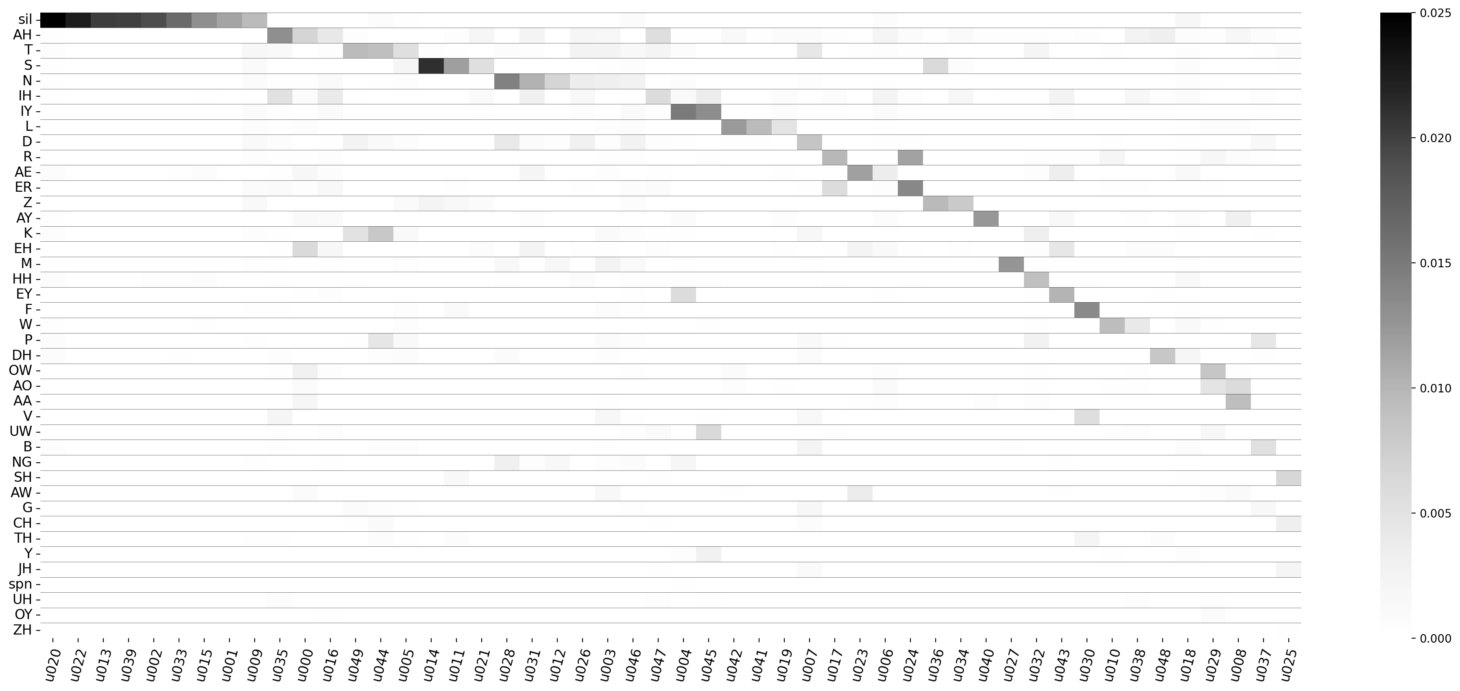
\includegraphics[width=1\linewidth]{figures/hubert-50-joint-byprob.png}
    \caption{HuBERT 模型、分群數為 50 之離散單元與音位標註的共同機率分佈圖}
    \label{fig:hubert-50-joint-byprob}
\end{figure}

        圖中的縱軸表示各個音位,橫軸表示各個離散單元。在這張圖中,縱軸的音位是按照其邊際機率 \(p_y(i)\) 由高至低排序;橫軸的離散單元則是依據其對應的最高機率音位 \(y^\ast(j)\) 的縱軸排序位置進行排列。\footnote{如果兩個離散單元 \(j_1\) 和 \(j_2\) 對應到相同的音位 \(y^\ast = y^\ast(j_1) = y^\ast(j_2)\),則依照機率值 \(p_{yz}(y^\ast, j_1)\) 和 \(p_{yz}(y^\ast, j_2)\) 由高到低進行排序,對於多個離散單元的情況以此類推。} 這樣可以在熱圖上顯示由左上至右下的對應關係。

        藉由熱圖的幫助,我們不僅可以更加完整清晰的觀察離散單元與音位標註之間的關係,對於純度大小的意義也可以從此圖上有更具體的了解:

        \begin{enumerate}
            \item 將每個直行(Column)取最大值相加後的總和即為音位純度。如果每個離散單元與音位都相對集中,則可以得到較高的音位純度。且如同指標說明的小節所述,當分群數量增加時,音位純度能夠在每個直行上取到更多的機率值總和。最極致的情況是,當分群數量與音框數量相同,音位純度可以達到 100\%。這些性質透過熱圖的可視化呈現,可以被更直觀的說明。

            \item 將每個橫列(Row)取最大值相加後的總和則是分群純度。如果每個音位都恰好可以很集中的對應到少數幾個離散單元,則此數值將較高,每個橫列最高可以貢獻的值為該音位出現的機率 $p_{y}(i)$。同樣的,當分群數量增加時,隨著直行數目的增多,單看每一個音位對應的橫列,會發現每個格子的機率值隨之被稀釋。受到音位標註類別數的限制,分群純度最高只能取 41 個 $p_{yz}$ 值的總和,使得單位純度因而明顯降低。
        \end{enumerate}

        此外,比起只有音位與分群純度兩個數字,機率熱圖不但可以呈現純度指標的綜觀解釋性意義,我們還可以分門別類對個別的音位與離散單元進行細部探討。畢竟,模型的虛擬標註與實際人類給予的標註資料並不能總是完美而集中的互相對應。我們想知道的細部觀察可分為兩個層面:

        \begin{enumerate}
            \item 從離散單元的角度出發,每個單元 $j$ 所對應的音位是如何的集中,因而多能夠代表這個單元中最高機率的音位 $y^*(j)$?如果恰巧該單元對應的音位條件機率分佈 $p_{y|z}(i|j)$ 較為分散,那與這個單元最相關,也就是條件機率前幾高的音位之間,又是否呈現特定關係?
            \item 反之從音位標註考慮,對於每個音位 $i$,觀察它所對應的離散單元集中程度,也就是離散單元條件機率分佈 $p_{z|y}(j|i)$ 得出的熵值 $H(z|y)$ ,可否觀察到特定一些音位較難或較易被離散單元集中歸類,進而推論模型是否善於辨認該音位的發音特性。
        \end{enumerate}

        接下來,我們將從綜觀的角度比較來自不同語音表徵與分群數的離散單元的純度和相互資訊數據,並輔以對應的機率熱圖佐證,觀察離散表徵在捕捉發音資訊方面的能力強弱。此後,分別從離散單元和音位兩個面向,藉助音位分類知識的幫助,進行細部觀察。最後將細部觀察的結論,重新對應回機率熱圖上的深淺規律,以對這些觀察的進行驗證。

\section{分析結果}

\subsection{綜觀分析}

  表 \ref{tab:single-cluster-results} 提供了不同語音表徵與分群數的純度和相互資訊的指標數據。

        首先,我們先比較同樣是分群數為 50 時,四種語音表徵的共同機率分佈熱圖,呈現在圖 \ref{fig:ch3-heatmap-model-comparison--part1} 中。從圖中可以明顯觀察到,HuBERT 和 CPC 在熱圖上具備較多較深且清晰的方塊,這表示音位與離散單元之間的對應相對 Wav2vec 2.0 與 LogMel 更為明確。這反映出 HuBERT 和 CPC 的離散表徵更擅長捕捉並區分音位之間的關係。此觀察也對應到這兩個模型較高的音位純度與相互資訊數值。

        接著考慮分群數的效應,我們進一步觀察分群表現最好的模型 HuBERT 在分群數為 50、100 和 200 的共同機率分佈熱圖。圖 \ref{fig:hubert-comparison} 是三者的比較結果,從圖中可以發現,在分群數愈多時,熱圖較深的區域愈是可以集中連成一條線,落在線外的色塊變得更少,但每個格子的機率值也隨之迅速降低。這個趨勢可以解釋為什麼表 \ref{tab:single-cluster-results} 中上升的音位純度與下降的分群純度,不過從表格中可以發現,其實相互資訊的數值仍是隨著分群數上升而提高的,也就是分群數多時,可以幫助提升離散單元與音位標註之間的相關性。

{

\begin{table}[!htbp]
    \centering
    \begin{subtable}[t]{\textwidth}
        \centering
        \begin{tabular}{|c|c|c|c|c|c|} \hline
                        & 音位純度   & 分群純度   & 音位熵    & 離散單元熵  & PNMI   \\ \hline
            HuBERT      &     0.5256 &     0.3382 &    3.3152 &      3.8681 & 0.4993 \\ \hline    %% 1.6552 h
            CPC         &     0.5188 &     0.3812 &    3.3146 &      3.7918 & 0.4992 \\ \hline    %% 1.6545 c
            Wav2vec 2.0 &     0.4006 &     0.2676 &    3.3152 &      3.8215 & 0.3706 \\ \hline    %% 1.2286 w
            LogMel      &     0.3253 &     0.1473 &    3.3158 &      3.8630 & 0.2647 \\ \hline    %% 0.8776 l 
        \end{tabular}
        \caption{分群數 = 50}
        \label{tab:ch3-clu050-phn}
    \end{subtable}

    \vspace{0.5cm}

    \begin{subtable}[t]{\textwidth}
        \centering
        \begin{tabular}{|c|c|c|c|c|c|} \hline
                        & 音位純度   & 分群純度   & 音位熵    & 離散單元熵  & PNMI   \\ \hline
            HuBERT      &     0.6097 &     0.2553 &    3.3152 &      4.5704 & 0.5786 \\ \hline    %% 1.9181 h
            CPC         &     0.5895 &     0.2674 &    3.3146 &      4.5034 & 0.5557 \\ \hline    %% 1.8418 c
            Wav2vec 2.0 &     0.4877 &     0.2118 &    3.3152 &      4.5284 & 0.4596 \\ \hline    %% 1.5235 w
            LogMel      &     0.3348 &     0.0931 &    3.3158 &      4.5591 & 0.2789 \\ \hline    %% 0.9247 l 
        \end{tabular}
        \caption{分群數 = 100}
        \label{tab:ch3-clu100-phn}
    \end{subtable}

    \vspace{0.5cm}

    \begin{subtable}[t]{\textwidth}
        \centering
        \begin{tabular}{|c|c|c|c|c|c|} \hline
                        & 音位純度   & 分群純度   & 音位熵    & 離散單元熵  & PNMI   \\ \hline
            HuBERT      &     0.6474 &     0.1644 &    3.3152 &      5.2681 & 0.6289 \\ \hline    %% 2.0849 h
            CPC         &     0.6098 &     0.1789 &    3.3146 &      5.1885 & 0.5882 \\ \hline    %% 1.9497 c
            Wav2vec 2.0 &     0.5427 &     0.1467 &    3.3152 &      5.2173 & 0.5188 \\ \hline    %% 1.7199 w
            LogMel      &     0.3474 &     0.0569 &    3.3158 &      5.2322 & 0.2955 \\ \hline    %% 0.9798 l 
        \end{tabular}
        \caption{分群數 = 200}
        \label{tab:ch3-clu200-phn}
    \end{subtable}

    \caption{四種語音表徵在不同分群數的純度與相互資訊數據}
    \label{tab:single-cluster-results}
\end{table}

}  % table
{

% \newcommand{\jeffheightt}[1]{\includegraphics[width=0.6\linewidth]{#1}}
\newcommand{\jeffheightt}[1]{\includegraphics[width=1\linewidth]{#1}}

\begin{figure}
     \centering
     \begin{subfigure}{\textwidth}  % [t]{\textwidth}
         \centering
         \jeffheightt{figures/hubert-50-joint-byprob--new1.png}
         \caption{HuBERT}
         \label{fig:ch3-heatmap-model--hubert-50-joint-byprob}
     \end{subfigure}
     \vfill

     \begin{subfigure}{\textwidth}  % [t]{\textwidth}
         \centering
         \jeffheightt{figures/cpc-50-joint-byprob.png}
         \caption{CPC}
         \label{fig:ch3-heatmap-model--cpc-50-joint-byprob}
     \end{subfigure}

     % \vfill
     % \begin{subfigure}{\textwidth}  % [t]{\textwidth}
     %     \centering
     %     \jeffheightt{figures/cpc-50-joint-byprob.png}
     %     \caption{CPC}
     %     \label{fig:ch3-heatmap-model--cpc-50-joint-byprob}
     % \end{subfigure}
     % \vfill
     % \begin{subfigure}{\textwidth}  % [t]{\textwidth}
     %     \centering
     %     \jeffheightt{figures/logmel-50-joint-byprob.png}
     %     \caption{LogMel}
     %     \label{fig:ch3-heatmap-model--logmel-50-joint-byprob}
     % \end{subfigure}
     \caption{不同語音表徵在分群數為 50 的共同機率分佈熱圖}
     \label{fig:ch3-heatmap-model-comparison--part1}
\end{figure}


\begin{figure}
    \ContinuedFloat
    % \setcounter{subfigure}{2}
     \centering
     % \begin{subfigure}{\textwidth}  % [t]{\textwidth}
     %     \centering
     %     \jeffheightt{figures/hubert-50-joint-byprob--new1.png}
     %     \caption{HuBERT}
     %     \label{fig:ch3-heatmap-model--hubert-50-joint-byprob}
     % \end{subfigure}
     % \vfill
     % \begin{subfigure}{\textwidth}  % [t]{\textwidth}
     %     \centering
     %     \jeffheightt{figures/w2v2-50-joint-byprob.png}
     %     \caption{Wav2vec 2.0}
     %     \label{fig:ch3-heatmap-model--w2v2-50-joint-byprob}
     % \end{subfigure}
     % \vfill
     
          \begin{subfigure}{\textwidth}  % [t]{\textwidth}
         \centering
         \jeffheightt{figures/w2v2-50-joint-byprob.png}
         \caption{Wav2vec 2.0}
         \label{fig:ch3-heatmap-model--w2v2-50-joint-byprob}
     \end{subfigure}
     
     \vfill
     \begin{subfigure}{\textwidth}  % [t]{\textwidth}
         \centering
         \jeffheightt{figures/logmel-50-joint-byprob.png}
         \caption{LogMel}
         \label{fig:ch3-heatmap-model--logmel-50-joint-byprob}
     \end{subfigure}
     \caption{不同語音表徵在分群數為 50 的共同機率分佈熱圖(續)}
     \label{fig:ch3-heatmap-model-comparison--part2}
\end{figure}

}  % heatmaps

{

% \newcommand{\jeffheightt}[1]{\includegraphics[width=0.6\linewidth]{#1}}
\newcommand{\jeffheightt}[1]{\includegraphics[width=0.85\linewidth]{#1}}

\begin{figure}
     \centering
     \begin{subfigure}{\textwidth}  % [t]{\textwidth}
         \centering
         \jeffheightt{figures/hubert-50-joint-byprob--new2.png}
         \caption{分群數 = 50}
         \label{fig:ch3-heatmap-cluster--hubert-50-joint-byprob}
     \end{subfigure}
     \vfill

     \begin{subfigure}{\textwidth}  % [t]{\textwidth}
         \centering
         \jeffheightt{figures/hubert-100-joint-byprob---new2.png}
         \caption{分群數 = 100}
         \label{fig:ch3-heatmap-cluster--hubert-100-joint-byprob}
     \end{subfigure}

    \vfill

     \begin{subfigure}{\textwidth}  % [t]{\textwidth}
         \centering
         \jeffheightt{figures/hubert-200-joint-byprob.png}
         \caption{分群數 = 200}
         \label{fig:ch3-heatmap-cluster--hubert-200-joint-byprob}
     \end{subfigure}

     \caption{HuBERT 模型在不同分群數的共同機率分佈熱圖}
     \label{fig:hubert-comparison}
\end{figure}

}
% 後面可以在有 unit 切入時,探討 given unit 時,為什麼分群數太多不好,而 100 又有什麼優於 50 的好處。(有必要再用 given phn 說明太分散)

        以上是不同離散表徵系統的離散單元對語音訊號給予虛擬標註時,對應音位標註是否明確的觀察。我們發現 HuBERT 是四種語音表徵之中效果最佳的,而分群數則是愈多愈好。

\subsection{以離散單元角度切入}  % 3 + 4 + 5  %%% 先看縱軸

  探討完綜觀機率分佈的比較,接著我們從離散單元的角度出發,基於離散單元進行統計觀察。首先,我們可以如同綜觀分析的探討方式,分別從模型與分群數量兩個變量切入,並對每個離散單元計算對應的條件音位熵 $H(y|z)$ 並畫出直方圖進行比較。

        圖 \ref{fig:hist-model} 可以觀察到四種模型在分群數都是 50 時的條件音位熵直方圖,從圖中可以發現 HuBERT 和 CPC 的音位熵相較於 Wav2vec 2.0 和 LogMel 偏低,也就是 HuBERT 和 CPC 每個離散單元對應的音位相較集中,與綜觀探討得到的觀察相符。
{

% \newcommand{\jeffheightt}[1]{\includegraphics[width=0.6\linewidth]{#1}}
\newcommand{\jeffheightt}[1]{\includegraphics[width=0.51\linewidth]{#1}}

 % \newcommand{\jjvfill}{\vspace{0.05cm}}\renewcommand{\arraystretch}{0.7} % 調整行高
 \newcommand{\jjvfill}{\vfill}

\begin{figure}
     \centering
     \begin{subfigure}{\textwidth}  % [t]{\textwidth}
         \centering
         \jeffheightt{figures/histo-phngivenunitent-hubert50-cnt.png}
         \caption{HuBERT}
         \label{fig:ch3-heatmap-model--hubert-50-joint-byprob-hist}
     \end{subfigure}
     \jjvfill

     \begin{subfigure}{\textwidth}  % [t]{\textwidth}
         \centering
         \jeffheightt{figures/histo-phngivenunitent-cpc50-cnt.png}
         \caption{CPC}
         \label{fig:ch3-heatmap-model--cpc-50-joint-byprob-hist}
     \end{subfigure}

     % \caption{不同語音表徵在分群數為 50 的條件音位熵直方圖}
     % \label{fig:hist-model}
% \end{figure}


% \begin{figure}
    % \ContinuedFloat
     % \centering
     \jjvfill

          \begin{subfigure}{\textwidth}  % [t]{\textwidth}
         \centering
         \jeffheightt{figures/histo-phngivenunitent-w2v2_50-cnt.png}
         \caption{Wav2vec 2.0}
         \label{fig:ch3-heatmap-model--w2v2-50-joint-byprob-hist}
     \end{subfigure}
     
     \jjvfill
     \begin{subfigure}{\textwidth}  % [t]{\textwidth}
         \centering
         \jeffheightt{figures/histo-phngivenunitent-logmel50-cnt.png}
         \caption{LogMel}
         \label{fig:ch3-heatmap-model--logmel-50-joint-byprob-hist}
     \end{subfigure}
     \caption{不同語音表徵在分群數為 50 的條件音位熵直方圖
     % (續)
     }
     % \label{fig:hist-model--part2}
     \label{fig:hist-model}
\end{figure}

}  % heatmaps


%%%%%
        圖 \ref{fig:hist-cluster} 則是比較 HuBERT 模型在分群數為 50、100 和 200 時的條件音位熵。需注意的是,由於此時離散單元數量不同,因此直方圖的縱軸改以比例數值呈現,亦即將數量分別除以 50、100 和 200 以進行公平的比較。從圖中可以觀察到,分群數愈多確實使整體條件音位熵降低,也與綜觀探討得到的小結一致。

{

% \newcommand{\jeffheightt}[1]{\includegraphics[width=0.6\linewidth]{#1}}
\newcommand{\jeffheightt}[1]{\includegraphics[width=0.75\linewidth]{#1}}

\begin{figure}
     \centering
     \begin{subfigure}{\textwidth}  % [t]{\textwidth}
         \centering
         \jeffheightt{figures/histo-phngivenunitent-hubert50.png}
         \caption{分群數 = 50}
         \label{fig:ch3-heatmap-cluster--hubert-50-joint-byprob-hist}
     \end{subfigure}
     \vfill

     \begin{subfigure}{\textwidth}  % [t]{\textwidth}
         \centering
         \jeffheightt{figures/histo-phngivenunitent-hubert100-prob.png}
         \caption{分群數 = 100}
         \label{fig:ch3-heatmap-cluster--hubert-100-joint-byprob-hist}
     \end{subfigure}

    \vfill

     \begin{subfigure}{\textwidth}  % [t]{\textwidth}
         \centering
         \jeffheightt{figures/histo-phngivenunitent-hubert200-prob.png}
         \caption{分群數 = 200}
         \label{fig:ch3-heatmap-cluster--hubert-200-joint-byprob-hist}
     \end{subfigure}

     \caption{HuBERT 模型在不同分群數的條件音位熵直方圖}
     \label{fig:hist-cluster}
\end{figure}

}

        接著,由於本小節基於離散單元的角度,我們仿照前作如 SpeechTokenizer \cite{zhang2024speechtokenizer}、DinoSR \cite{liu2024dinosr} 的作法,將熱圖改以 $p_{y|z}(i|j)$ 呈現,即對每個直行進行標準化得到條件機率,以顯示每個單位對應到哪個音位,探討這種對應分佈是如何的集中或分散。

% /////////////
\begin{figure}
    \centering
    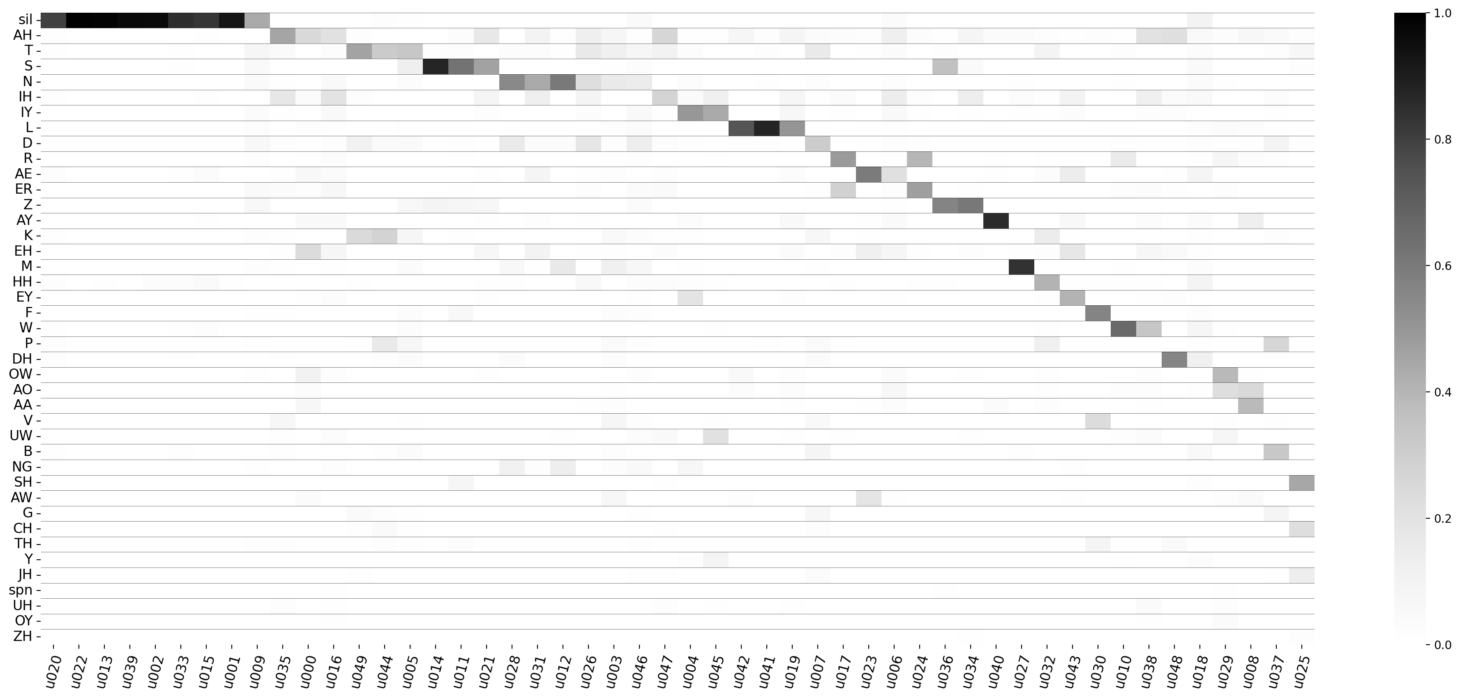
\includegraphics[width=1\linewidth]{figures/11111111.png}
    \caption{HuBERT 模型、分群數為 50 之 $p_{y|z}(i|j)$ 條件機率分佈圖}
    \label{fig:hubert-50-givenunit-byprob}
\end{figure}
        觀察圖 \ref{fig:hubert-50-givenunit-byprob} 中由左上而右下角對應的連線區域,首先我們會在左上方觀察到一條明顯較深的區域,也就是模型會安排一定數量的離散單元用以對應實際上並非音位的音位標註 sil。此外,我們還可以在連線區域之外觀察到一些零星的色塊,在此指示存在不少離散單元,它們對應的音位是相比較為分散的,也因此使得音位純度無法到達 100\%。

        不過,如果我們嘗試觀察這些將離散單元對應機率分散出去的音位,藉助語音學的知識可以觀察到一些有趣的發現:這些音位彼此之間在發音上具有很強的關聯性,幾乎與語音學提供的分類是對應的。 


        \begin{figure}
            \centering
            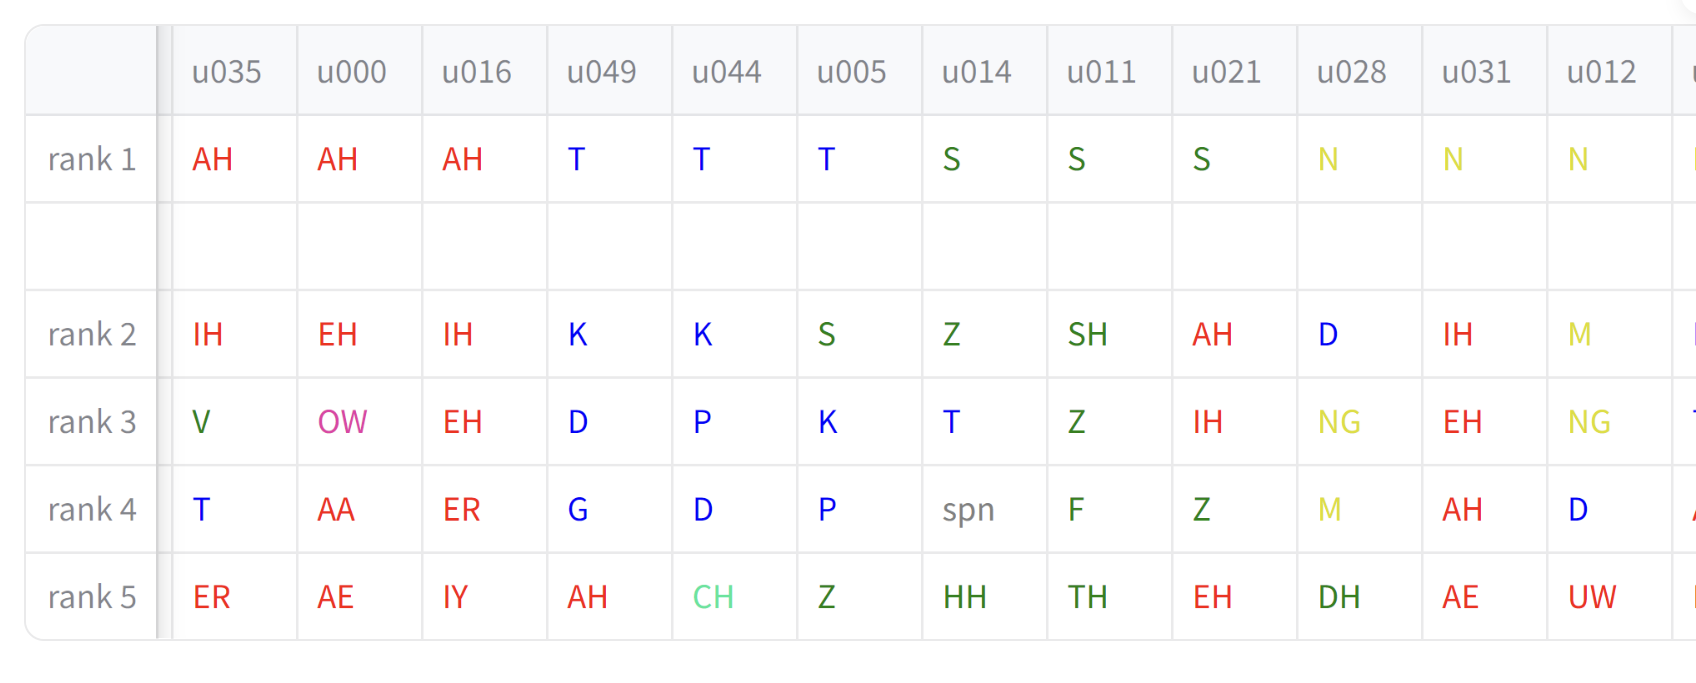
\includegraphics[width=1\linewidth]{figures/unit_rank_phn.png}  % figures/unit_perspective.png
            \caption[]{
 HuBERT 模型、分群數為 50 之部分離散單元所對應的前五高機率音位
% 。圖中的方框、圓圈等形狀
}
                                          % 表示輔音發聲部位,外框顏色則表示清濁音。注意元音都屬於濁音
                                          (音位分類以顏色標示區分)
            \label{fig:unit-to-phn-rankings}
        \end{figure}
        
\begin{figure}
    \centering
    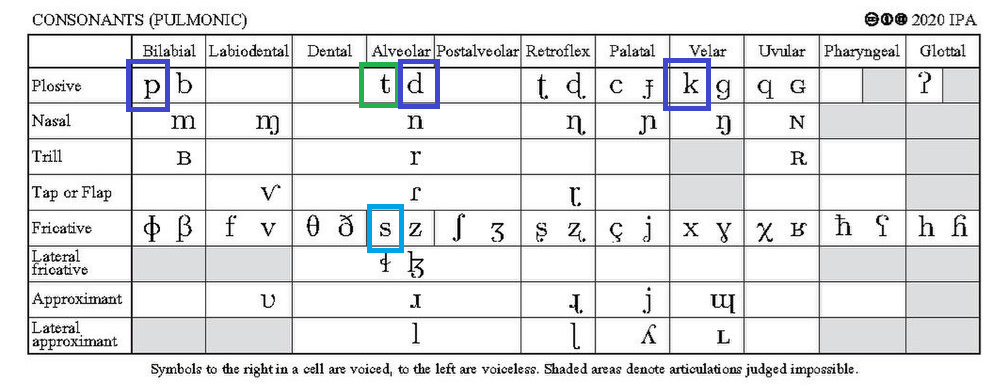
\includegraphics[width=1\linewidth]{figures/ipa_similarity.png}
    \caption[]{
國際音標表的輔音表格,說明離散單元}
                                                                對語音聲學特徵的捕捉並不僅限單一面向
    \label{fig:ipa-cons-table-sim}
\end{figure}

        為了方便說明,我們將熱圖上各個離散單元排名前五高的對應音位另外列表呈現在圖 \ref{fig:unit-to-phn-rankings} 中,並用顏色標明各音位所屬的音位分類。從表中大致可以看出前幾高機率的音位所屬的類別確實是相近的。而且即便不是同一個音位分類,這些音位在語音學中,仍有其他層面 --- 如發音部位和清濁音 --- 的相似性,還是可以將各離散單元的前幾高音位中找出共通點。

        事實上,為了作圖與統計方便,語音處理相關研究 \cite{10097097, abdullah23_interspeech} 對音位的歸類是相對簡化的。根據語音學的知識,音位之間的分組方式並不只一種,而本研究著重的分類方式僅是以「發音方式」為主。
例如 05 號單元對應的前兩名 /t/ 和 /s/ 雖然並不屬於同一個發聲方式,因而被分成兩個類別,但如果參考圖 \ref{fig:ipa-cons-table-sim} 的國際音標表 \footnote{表中的每個橫列約等於本論文與相關研究\cite{10097097, abdullah23_interspeech} 使用的「發音方式」分類法,而每個用直線隔開的直行則是指「發音部位」相同,同一個格子的左右則是呈現一對清濁音音位。},會發現它們都屬於「齒音」,亦即它們的「發音部位」是相同的。換言之這些離散單元捕捉到的語音特性是多個面向的,並不僅限於單一的分類方式,而是可以對應到國際音標表上至少兩個維度以上的類型。

        透過以上的觀察,因此我們有足夠的理由重新對熱圖的縱軸重新排列,並按照語音學分類進行分組,來觀察這些離散單元是如何指示出音位之間的相似性,區分出同個音位、同類發音,或者如何被混淆為其他類別。  
%,而這些類別是否有某些特徵,最後這樣的現象是否只在單一模型出現,抑或是在不同的離散單元系統都會發生。

\begin{figure}
    \centering
    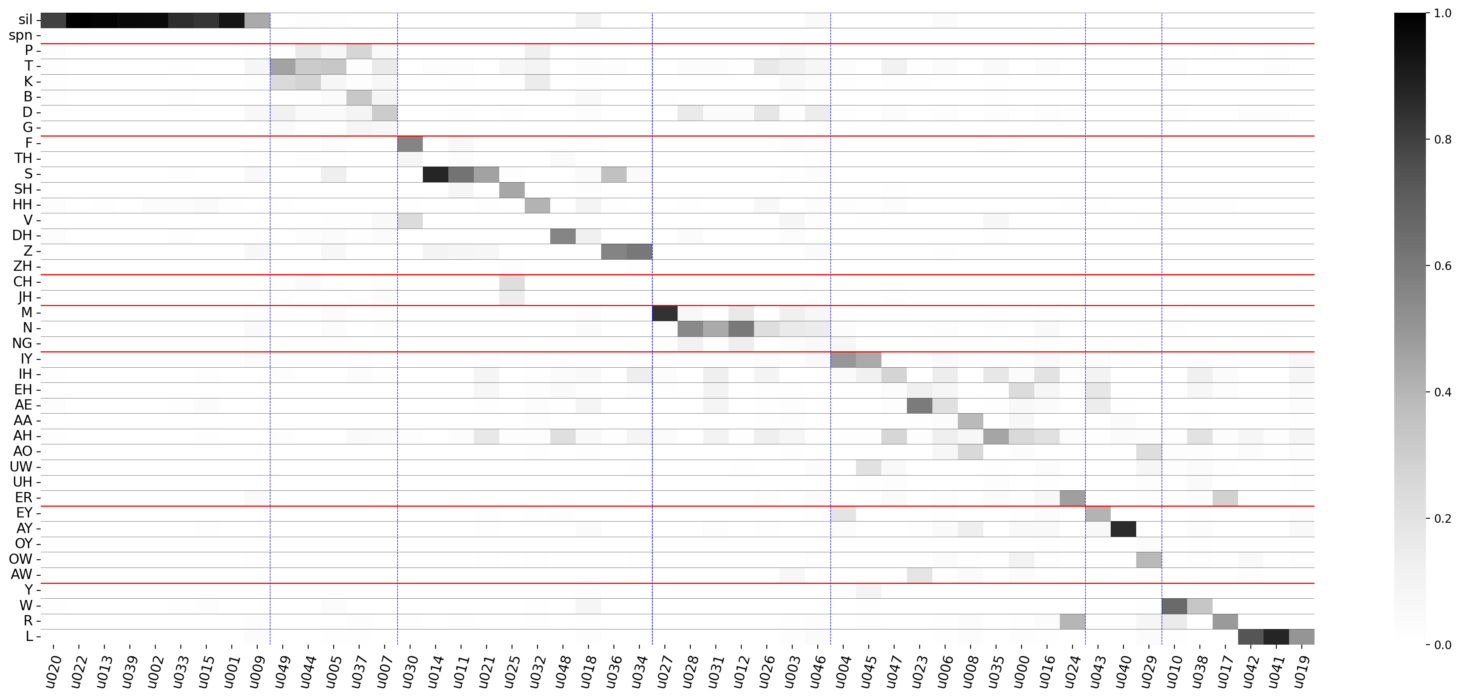
\includegraphics[width=1\linewidth]{figures/hubert-50-givenunit-byphn.png}
    \caption[]{% \medskip % \small
        HuBERT 模型、分群數為 50 之離散單元與音位標註的條件機率,}
                                                    依照韋氏(Wells) \cite{wells_phonetic_2022} 論文與音位類別排序的分佈圖
    \label{fig:hubert-50-givenunit-byphn}
\end{figure}

        圖 \ref{fig:hubert-50-givenunit-byphn} 的分組順序是依照韋氏(Wells) \cite{wells_phonetic_2022} 論文中的出現順序排列,而組別內則是清音在上、濁音在下,而同樣清濁音則是以發音位置由前往後排列。除了縱軸上按照音位本身特性分組,依循純度中使用的「代表音位」 $i^\ast$ 概念,我們同樣也對每個離散單元的代表音位排序,並且也依照這些代表音位進行分組觀察。

        最後,對於每個離散單元 $j$ 與對應的最高機率音位 $y^*(j)$,為了統計該單元 $j$ 除了 $y^*(j)$ 以外,是否也給予與 $y^*(j)$ 同音位分類 $\kappa^*(j)$ 的其他音位較高的機率值,我們藉由調整純度的計算式,但將音位標註改為音位分類並重新統計,以方便我們比較離散單元「對音位分類歸類能力」的強弱。計算方式為:

        如果 $y^*(j) \in \kappa^*(j)$,$ \kappa^*(j) = \{y^*(j), y', y'', \cdots\cdots\}$  是所有與  $y^*(j)$ 同音位分類的音位,則將這些音位的標註改為 $ \kappa^*(j) $ ,統計音位分類純度
\begin{align}
    \mathbb{E}_{p_z(j)}\left[p_{ \kappa|z}( \kappa^*(j)|j) \right]
\end{align}
與音位分類的分群純度
\begin{align}
    \mathbb{E}_{p_ \kappa(\kappa^*)}\left[p_{z| \kappa}(z^*( \kappa^*)|\kappa^*) \right]
\end{align}
以此刻劃離散表徵是否能歸類語音學上相似的發音特徵。


\begin{figure}
        \centering
        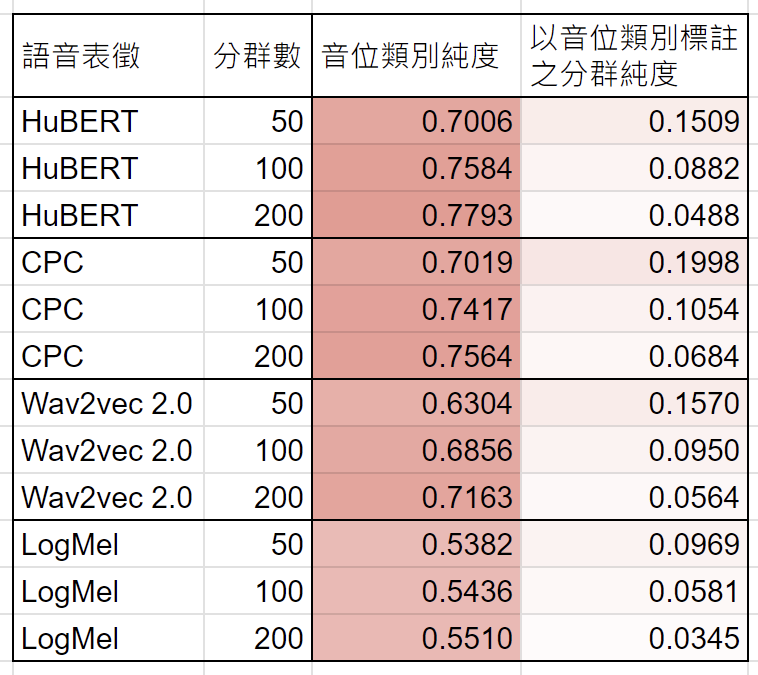
\includegraphics[width=0.55\linewidth]{figures/pcls-pur.png}
    \caption{以音位分類為標註計算,四種語音表徵在不同分群數的純度數據}
    \label{fig:pcls}
    \end{figure}

        圖 \ref{fig:pcls} 是不同離散表徵在音位分類純度與對應的分群純度結果。由表中可以再次確認,HuBERT 的離散單元不但能夠很好的區分出音位,即便某些離散單元沒有集中分到特定音位之上,也可以很不錯的給予同類別的音位較高的機率值,以得到較高的音位分類純度數值。

% sil 沒有必要寫了!(說不定 purity cls 也可以拿掉)

\subsection{以音位角度切入}

  接著,我們改從音位的角度切入,觀察每個音位所對應的離散單元條件熵 $H(z|y)$,以探討不同音位之間是否有特定音位較容易或較難以被離散表徵歸類。表 \ref{fig:phn-specials} 分別呈現了不同模型在分群數為 50 和 100 時,離散單元熵最高與最低的幾個音位。雖然沒有特別明顯的趨勢,但可以大致看到以下幾點:

\begin{itemize}
    \item 熵值較低的音位有 AA、EY、F、ZH、SH、S 等,其中 F、ZH、SH、S 皆屬於擦音。
    \item 熵值較高的音位有 spn、AH、IH、T、D 等,其中 T、D 屬於塞音。  % 機率高低先跳過了
\end{itemize}

        整體而言,擦音的離散單元相對較為集中,而塞音則相對較為分散。至於其他如 AH、IH 等高熵值的元音音位,推測其原因可能是它們本身在不同發音情境下音色的變化相對於 AA、EY 等較大,因而較難集中於某幾個離散單元。這個趨勢在不同的語音表徵和分群數下約略存在,但以 HuBERT 和 CPC 較為明顯。


{

% \newcommand{\jeffheightt}[1]{\includegraphics[width=0.6\linewidth]{#1}}
\newcommand{\jeffheightt}[1]{\includegraphics[width=1\linewidth]{#1}}

\begin{figure}
     \centering
     \begin{subfigure}{\textwidth}  % [t]{\textwidth}
         \centering
         \jeffheightt{figures/phnrank50.png}
         \caption{分群數 = 50}
         \label{fig:phn-specials-clu50}
     \end{subfigure}
     \vfill

     \begin{subfigure}{\textwidth}  % [t]{\textwidth}
         \centering
         \jeffheightt{figures/phnrank100.png}
         \caption{分群數 = 100}
         \label{fig:phn-specials-clu100}
     \end{subfigure}

     \caption{不同語音表徵在分群數為 50 和 100 時,離散單元條件熵最高與最低的音位}
     \label{fig:phn-specials}
\end{figure}

}



\begin{figure}
    \centering
    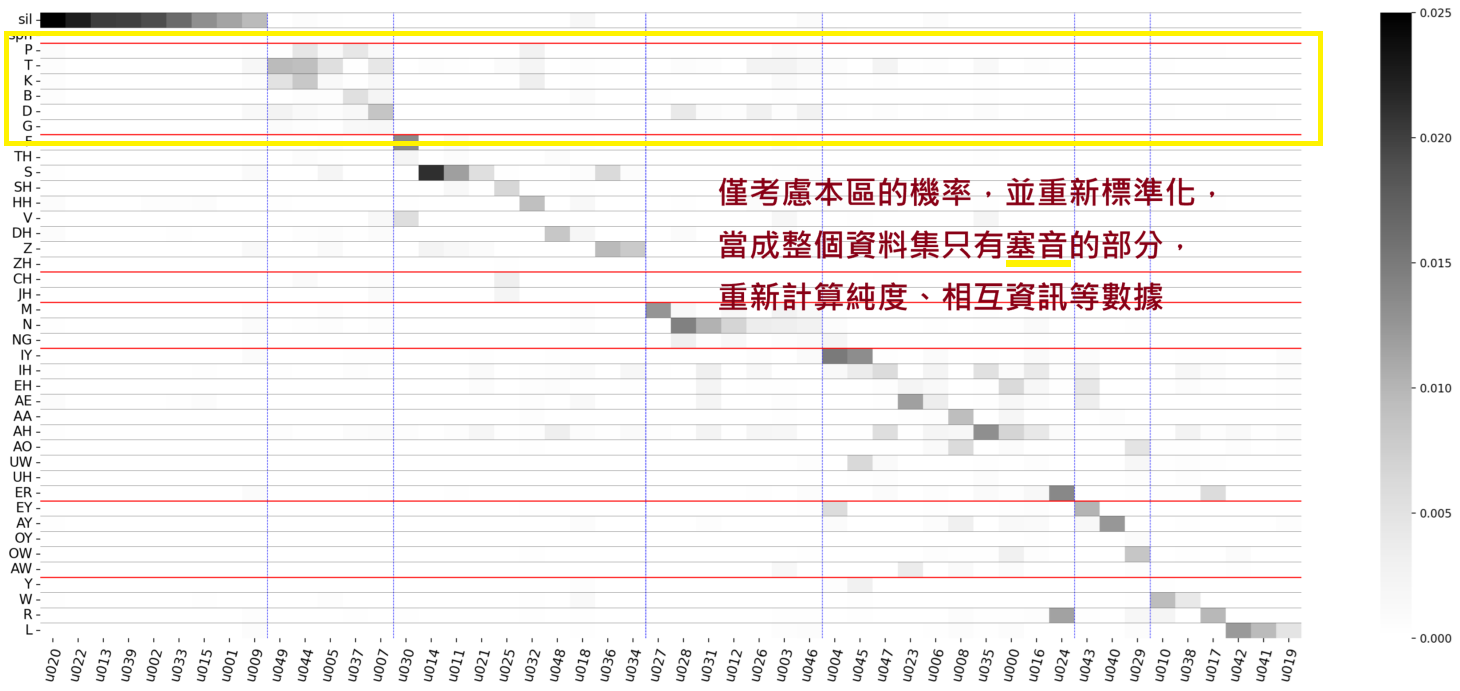
\includegraphics[width=1\linewidth]{figures/better-demo-splitter.png}
    \caption{對共同機率分佈按照音位分類分別計算純度作法示意圖}
    (以塞音舉例,同樣的作法對紅線分開的八塊區域分別計算)
    \label{fig:demo-splitter}
\end{figure}


        為了進一步驗證不同音位分類之間的差異,我們再度引用純度與相互資訊的計算公式,但將統計範圍限定為不同音位分類,分別計算針對每個音位分類的純度與相互資訊。換言之,我們共同機率分佈圖 $p_{yz}$ 按照圖 \ref{fig:demo-splitter} 的紅色水平線分成八塊後,重新標準化並各自計算純度與相互資訊,相當於將原本的語音音框按照音位分類分成八組各自統計這些指標。如此一來,我們既可以依據每個音位分類觀察在不同離散表徵對該類別的表現差異,也可以比較不同音位分類彼此的整體趨勢,歸納音位分類本身發音特徵被捕捉的難易程度。

\begin{figure}
    \centering
    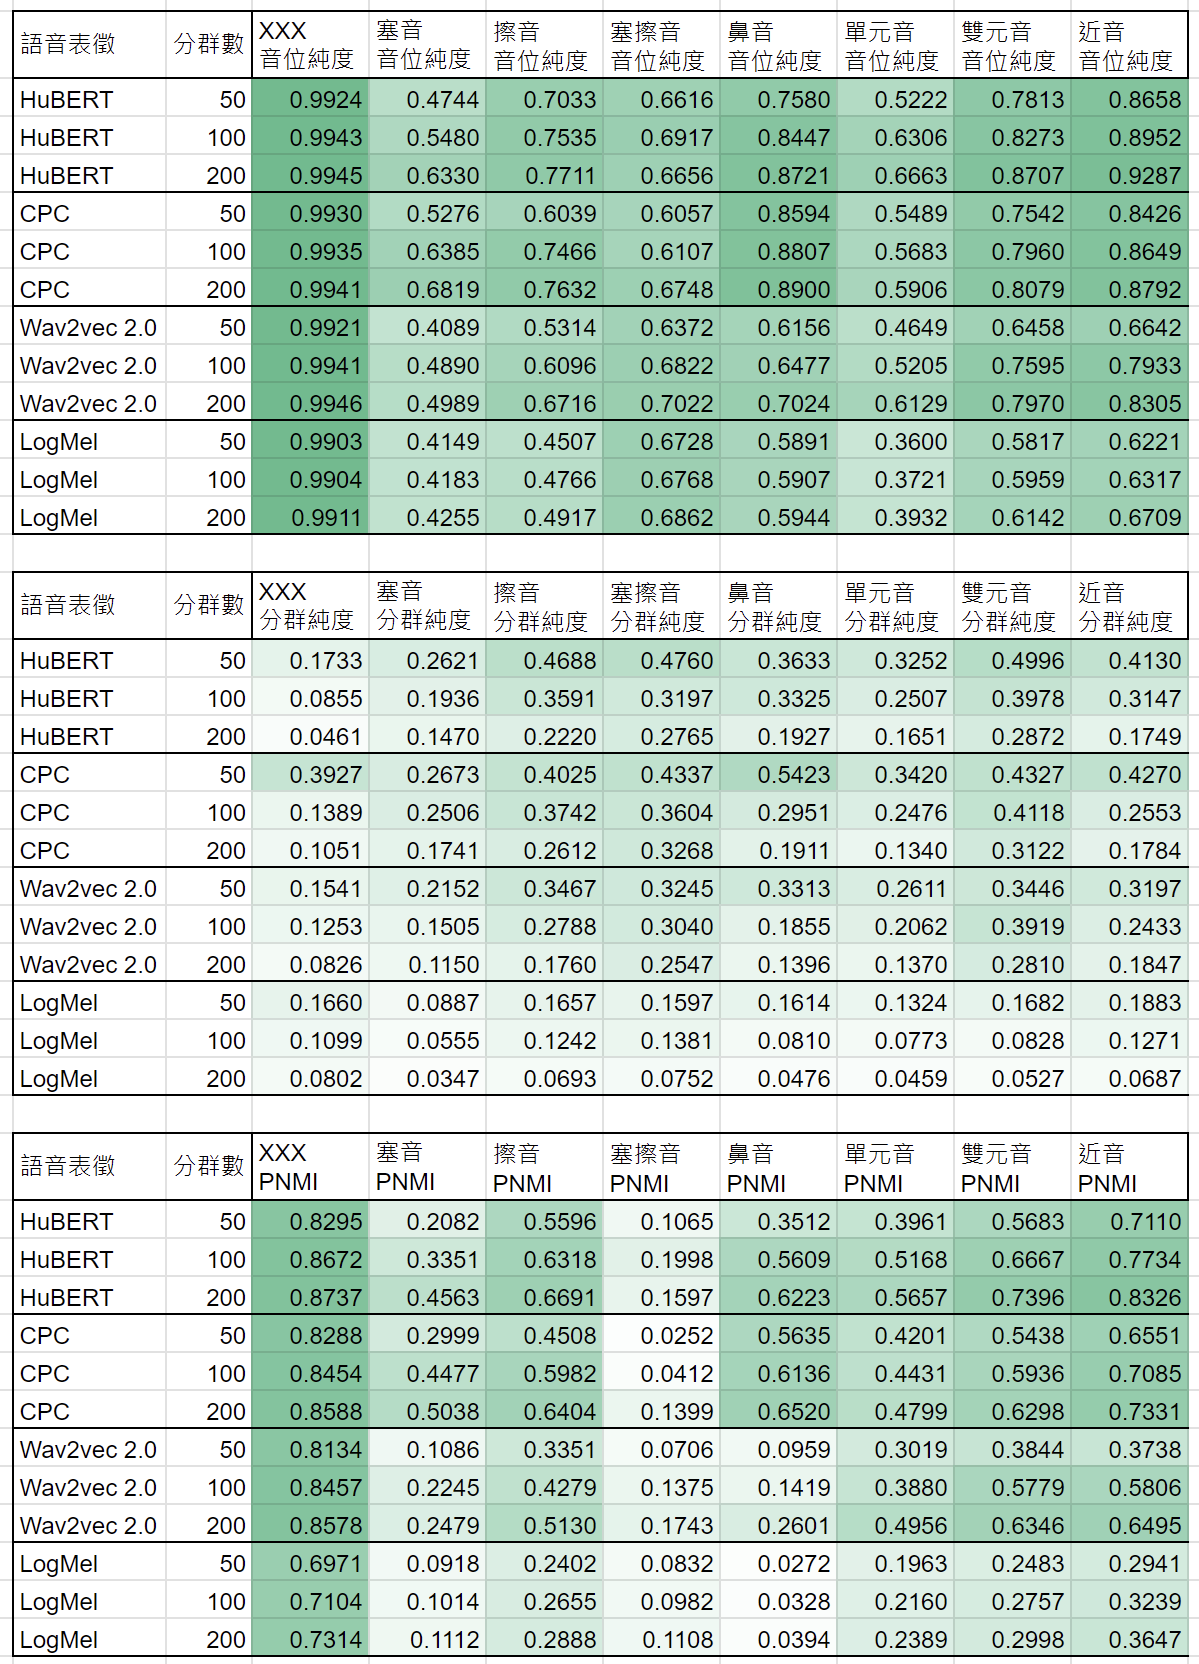
\includegraphics[width=1\linewidth]{figures/pur-of-each-cls-xls.png}
     \caption{按照音位分類分開各自計算的純度與相互資訊}
     \label{fig:pur-of-each-cls}
\end{figure}


        表 \ref{fig:pur-of-each-cls} 中呈現了這些模型的比較數據。由圖中依然可以觀察到 HuBERT 優於其他模型,且分群數愈多時相互資訊與音位純度愈高,這些趨勢與前面所有的觀察結論一致。

        從音位分類之間的比較,我們可以觀察到:撇除非音位(表格中的「XXX」)類別不考慮,\footnote{因其只有 sil 一類標註,因此相互資訊和純度相當高。}可以確定塞音和塞擦音的純度較低,確實是較難以集中歸類的音位分類;而近音、雙元音和擦音則純度相對較高,這也驗證為什麼它們的離散單元熵值較低且分佈較為集中。

\subsection{整體熱圖驗證}

{

% \newcommand{\jeffheightt}[1]{\includegraphics[width=0.6\linewidth]{#1}}
\newcommand{\jeffheightt}[1]{\includegraphics[width=0.75\linewidth]{#1}}

\begin{figure}
     \centering
     \begin{subfigure}{\textwidth}  % [t]{\textwidth}
         \centering
         \jeffheightt{figures/badhub50.png}
         \caption{HuBERT + 分群數 = 50}
         \label{fig:ch3-badhub50}
     \end{subfigure}
     \vfill

     \begin{subfigure}{\textwidth}  % [t]{\textwidth}
         \centering
         \jeffheightt{figures/badhub100.png}
         \caption{HuBERT + 分群數 = 100}
         \label{fig:ch3-badhub100}
     \end{subfigure}

    \vfill

     \begin{subfigure}{\textwidth}  % [t]{\textwidth}
         \centering
         \jeffheightt{figures/badcpc100.png}
         \caption{CPC + 分群數 = 100}
         \label{fig:ch3-badcpc100}
     \end{subfigure}

     \caption{熱圖驗證塞音、塞擦音較難以被離散單元歸類,}
     注意塞擦音在 HuBERT + 分群數 = 50 和 CPC + 分群數 = 100 \\
     甚至可能沒有專門的離散單元以其為代表
     \label{fig:finalObserv}
\end{figure}

}


{

% \newcommand{\jeffheightt}[1]{\includegraphics[width=0.6\linewidth]{#1}}
\newcommand{\jeffheightt}[1]{\includegraphics[width=0.75\linewidth]{#1}}

\begin{figure}
     \centering
     \begin{subfigure}{\textwidth}  % [t]{\textwidth}
         \centering
         \jeffheightt{figures/goodhub50 - 複製.png}
         \caption{HuBERT + 分群數 = 50}
         \label{fig:ch3-goodhub50}
     \end{subfigure}
     \vfill

     \begin{subfigure}{\textwidth}  % [t]{\textwidth}
         \centering
         \jeffheightt{figures/goodhub100 - 複製.png}
         \caption{HuBERT + 分群數 = 100}
         \label{fig:ch3-goodhub10}
     \end{subfigure}

    \vfill

     \begin{subfigure}{\textwidth}  % [t]{\textwidth}
         \centering
         \jeffheightt{figures/goodcpc100 - 複製.png}
         \caption{CPC + 分群數 = 100}
         \label{fig:ch3-goodcpc10}
     \end{subfigure}

     \caption{熱圖驗證擦音、雙元音與近音的特徵較明顯}
          \label{fig:finalObserv2}
\end{figure}

}

  最後,參考韋氏(Wells) \cite{wells_phonetic_2022} 的研究方法,我們探討不同音位分類中音位與離散單元的對應關係。比起直接看離散單元的編號,我們改對機率熱圖進行分區觀察以確認趨勢。為了同時對比語音表徵與分群數兩個變因造成的差異,我們比較 HuBERT 分群數 50 和 100 以及 CPC 分群數 100 的機率熱圖,並參考 SpeechTokenizer \cite{zhang2024speechtokenizer} 和 DinoSR \cite{liu2024dinosr} 的作法,以 $p_{y|z}(i|j)$ 呈現,確認離散表徵對於音位的歸類效果,最終驗證前述觀察。圖 \ref{fig:finalObserv} 中框出的區域為前述觀察到較為分散的塞音與塞擦音,這些區域確實顏色較淺(塞擦音在 HuBERT + 分群數 = 50 和 CPC + 分群數 = 100 甚至可能沒有專門的離散單元以其為代表),證明其語音特徵歸類的確較為困難;而圖 \ref{fig:finalObserv2} 中框出的區域則是離散表徵歸類較集中的擦音、雙元音與近音,這幾區的色塊如前面推論所預測的較為明顯,屬於容易區分的音位分類。

% 最後,關於非音位的語音訊號,觀察這些模型的等效花費多少比例的離散單元去代表這些非音位的資訊,可以發現 HuBERT 雖然擷取音位的整體表現比較好,但也耗費了不低比例的單元去編碼非音位的資訊。

\section{本章總結}

  本章節探討以音框為單位取出的語音離散表徵與對應的音位標註之間的關係。我們從純度的計算開始,對整個機率熱圖進行可視化分析,並透過語音知識的協助,尤其是對音位的分類,將原先約 40 類的獨立標註進行更深入的特性分析。

        透過這些探討,從語音學的角度,我們發現塞音的離散單元分佈較為分散,而擦音則較為集中。同時,藉由比對不同模型間的數據表現差異,也確認了 HuBERT 模型的離散表徵在各項數據中與音位之間的相似性最為明顯。因此,進一步印證了 HuBERT 為何是抽取語音離散表徵時最常使用的模型,並常被無文字架構所使用。

        然而,單一離散表徵僅能代表 10 或 20 毫秒的語音訊號,而音位的長度經常佔據不只一個離散表徵。因此,下一章節將嘗試進一步組合多個離散表徵成為符記,分析它們與音位之間的關係。

%        從統計數據出發,我們針對共同機率分佈的各個面向,配合了語音學知識的分類進行了細部探討,發現了 hunert 模型怎樣怎樣,而這件事可能在其他的模型之中差不多是 holid 住的。然後,因為 hunert 本身捕捉的各項純度與 MI 明顯較高,以此可以驗證為什麼 HuBERT 的離散單元可以在無文字架構內被當成類似音位或文字的表徵,並進而套用於語音語言模型的訓練上,同時為許多做語音模型解釋性的作品所關注citehao。
